\documentclass[a4paper,11pt]{article}
\usepackage[dvips]{graphicx}
\usepackage[T1]{fontenc}
\usepackage[utf8]{inputenc}
\usepackage[french]{babel}
\usepackage{lmodern} \normalfont
\DeclareFontShape{T1}{lmr}{bx}{sc}{<-> ssub * cmr/bx/sc}{}
\usepackage{textcomp}
\usepackage{fixltx2e}
\usepackage{exptech} % inclusion du style immposé
\usepackage{amsmath}
\usepackage{amssymb}
\usepackage{graphicx}
\usepackage{wrapfig}
\usepackage{subcaption}
\usepackage{listings}
\usepackage{color}
\usepackage{pdfpages}
\usepackage[colorlinks=true,
            linkcolor=blue,
            bookmarksnumbered=true,
            pdftitle={Report},
            pdfauthor={Antoine C., Hoel K.},
            pdfborder={0 0 0},
            pdfsubject={mittelwerk}]{hyperref}

\usepackage{fancyvrb} % for verbatim boxes

\title{\textbf{Contrôleurs dans l'espace}}
\author{Julien \textsc{Bouvet}, Antoine \textsc{Chenon}, Mikaïl \textsc{Demirdelen}, Hoel \textsc{Kervadec}
        \\
        Encadrants : Loic \textsc{Helouet}, Yann \textsc{Ricquebourg}}
\date{Juin 2014}
\markright{Contrôleurs dans l'espace}

\begin{document}
\thispagestyle{empty}

\maketitle
\begin{abstract}
    Parti d'un simulateur de vol spatial, nous avons créé une chaîne d'outils et un nouveau langage permettant de facilement automatiser les vaisseaux du dit simulateur, afin d'obtenir un démonstrateur visuel pour la théorie du contrôle, et ainsi faciliter l'illustration de concepts plus abstraits.
\end{abstract}

%\tableofcontents %A utiliser que pour la rédaction

%\setlength{\parskip}{5pt}

\section{Présentation du sujet}
    \subsection{Contexte}
        La théorie du contrôle a comme objet l'étude du comportement de systèmes dynamiques paramétrés en fonction des trajectoires de leurs paramètres. Elle sert à analyser les trajectoires de systèmes commandés.

        Ce domaine peut être utilisée de différentes manières : amener le système d'un état initial à un état final (l'objectif) ou assurer que le système ne se retrouve pas en mauvaise configuration...

    \subsection{Orbiter}
<<<<<<< HEAD
        Orbiter\footnote{\url{http://orbit.medphys.ucl.ac.uk/}} est un simulateur de vols spatiaux, développé par le Dr Martin \textsc{Schweiger}, qui était parti du constat que la simulation spatiale manquait cruellement d'un simulateur respectant les lois de la physique.
=======
        Orbiter\footnote{\url{http://orbit.medphys.ucl.ac.uk/}} est un simulateur de vols spatiaux, développé par Dr Martin SCHWEIGER, qui était parti du constat que la simulation spatiale manquait cruellement d'un simulateur respectant les lois de la physique.
>>>>>>> 447a0a4bf6d3335342ebd91ab2b01ea02587f4f8

        \begin{figure}[!h]
            \begin{center}
                
\includegraphics[width=0.7\textwidth]{img/orbiter_logo.png}
            \end{center}
        \end{figure}

        La première version fut publiée le 27 novembre 2000, et la dernière version stable en date est la version 2010.

<<<<<<< HEAD
        Malgré le succès rencontré par le simulateur et les nombreuses demandes d'ouverture du code\footnote{D'un point de vue open source}, l4quteur a toujours refusé de le faire, et a préféré à la place publier une API, afin tout de laisser la possibilité aux utilisateurs d'orbiter de développer ses propres modules, vaisseaux, etc.

        Orbiter possède de base de nombreux vaisseaux, et un grand nombre de missions différentes, allant des missions historiques, aux plus futuristes. Cette grande variété en fait un outil idéal pour apprendre des concepts de la physique en s'amusant, et peut être une excellence base pour servir de démonstrateur.

    \subsection{La théorie du contrôle}
        La théorie du contrôle recoupe l'ensemble des disciplines qui consistent à asservir un système, et à lui permettre de s'auto-gérer: c'est la base du pilotage automatique.
=======
        Malgré le succès rencontré par le simulateur et les nombreuses demandes d'ouverture du code\footnote{D'un point de vue open source}, l'auteur a toujours refusé de le faire, et a préféré à la place publier une API, afin tout de laisser la possibilité aux utilisateurs d'orbiter de développer ses propres modules, vaisseaux, etc.

        Orbiter possède de base de nombreux vaisseaux, et un grand nombre de missions différentes, allant des missions historiques, aux plus futuristes. Cette grande variété en fait un outil idéal pour apprendre des concepts de la physique en s'amusant, et peut être une excellence base pour servir de démonstrateur.

    \subsection{La Théorie du contrôle}
        La Théorie du contrôle recoupe l'ensemble des disciplines qui consistent à asservir un système, et à lui permettre de s'auto-gérer: c'est la base du pilotage automatique.
>>>>>>> 447a0a4bf6d3335342ebd91ab2b01ea02587f4f8

        Un des principe les plus simples est la boucle de contrôle: en se basant sur plusieurs variables (par exemple: la puissance d'un réacteur, vitesse, altitude, ...), et en les comparants à des objectifs, nous pouvons adapter cette puissance afin de minimiser l'écart entre l'objectif et l'état courant du système.

        \begin{figure}[!h]
            \begin{center}
                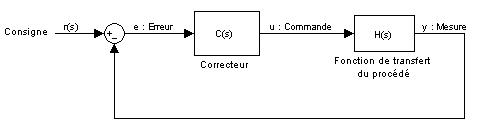
\includegraphics[width=1\textwidth]{img/boucle_controle.jpg}
                \caption{Exemple de système bouclé simple.}
            \end{center}
        \end{figure}
        
        Afin d'asservir le système, il est possible d'utiliser des automates, qui se chargeront de lire son état et d'opérer les commandes nécessaires pour se rapprocher du résultat souhaité.

<<<<<<< HEAD
        Parti du constat que Orbiter est un outil ludique et visuel, il a été proposé dans cette étude de créer une chaîne d'outils permettant d'automatiser facilement des vaisseaux d'Orbiter à l'aide de boucles de contrôles, évitant ainsi d'éditer leur code souvent complexe.
=======
        Parti du constat que Orbiter est un outil ludique et visuel, il a été proposé, dans cette étude, de créer une chaîne d'outils permettant d'automatiser facilement des vaisseaux d'Orbiter à l'aide de boucles de contrôles, car, de base, nous pouvons juste contrôler le vaisseau au clavier.
>>>>>>> 447a0a4bf6d3335342ebd91ab2b01ea02587f4f8

    \subsection{Objectifs initiaux}
        Pour automatiser les vaisseaux, nous avons été chargé de créer un nouveau langage, à la grammaire épurée, contenant des fonctions de base, et pouvant ainsi servir facilement de démonstrateur pour la théorie du contrôle.

        Le résultat pourrait servir dans des conférences ou des événements de vulgarisation scientifique, pour montrer facilement (et visuellement) les différentes manières d'aborder l'asservissement d'un vaisseaux.

        Le langage devait donc être très simple, et la chaîne logicielle la plus simple possible à utiliser, pouvant permettre à quiconque de créer ses propres automates.

        Par ailleurs, le travail devait être réutilisable, pour pouvoir être repris les années suivantes, et ainsi améliorer petit à petit ce compilateur.

\section{Réalisation pratique}
    \subsection{Architecture d'Orbiter}
        L'architecture du simulateur est propice à l'ajout de nouveaux modules: par exemple, tout les vaisseaux sont fournis sous forme de .dll. Ainsi, pour peu que l'on ai réussi à écrire et à compiler un nouveau module, il suffit de le copier dans le dossier adéquat pour être utilisable par Orbiter.
        
<<<<<<< HEAD
        Un vaisseau est donc écrit en C++, puis compilé vers une dll (par exemple, ShuttleA.dll). Ce code contient les fonctions régissant le comportement du vaisseau, ses spécificités ainsi que l'action des commandes manuelles\footnote{Orbiter s'utilisant au clavier et à la souris.} sur celui ci.
=======
        Un vaisseau est donc écrit en C++, puis compilé vers une dll (par exemple, ShuttleA.dll). Ce code contient les fonctions régissant le comportement du vaisseau, ses spécificités ainsi que l'action des commandes manuelles\footnote{Orbiter s'utilisant au clavier et à la souris, le "`joueur"' étant le pilote.} sur celui ci.
>>>>>>> 447a0a4bf6d3335342ebd91ab2b01ea02587f4f8
        
        On peut donc rajouter du code pour que le vaisseau se gère tout seul, créant ainsi notre automate, sans toucher à Orbiter en lui même. C'est cette création que nous allons dès à présent détailler.

    \subsection{Déroulement des opérations}
        Notre travail s'est porté sur un seul vaisseau (le ShuttleA), afin de nous concentrer sur la grammaire et notre compilateur. 
        
        Ce choix est lié au fait que le ShuttleA est composé d'une seule classe C++, ce qui nous permet une prise en main plus rapide et une intégration plus simple de notre automate. 
        
<<<<<<< HEAD
=======
        Une amélioration du projet pourrait être de supporter un plus grand nombre de vaisseaux (voire tous?) une fois que le langage est jugé suffisamment mature.

>>>>>>> 447a0a4bf6d3335342ebd91ab2b01ea02587f4f8
        \begin{figure}[!h]
            \begin{center}
                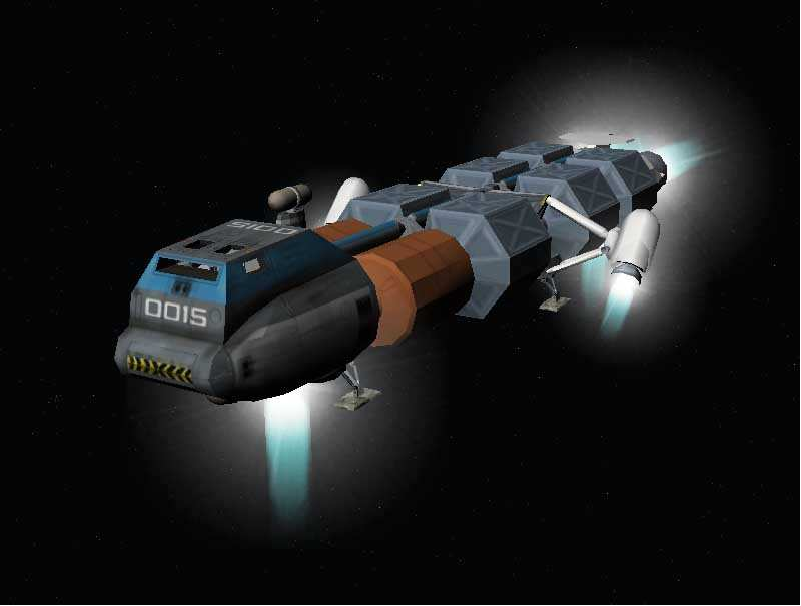
\includegraphics[width=0.5\textwidth]{img/shuttleA.png}
                \caption{Le ShuttleA, sujet de toute nos expériences.}
            \end{center}
        \end{figure}
        
        Une amélioration du projet pourrait être de supporter un plus grand nombre de vaisseaux (voire tous?) une fois que le langage est jugé suffisamment mature.



    \subsubsection{Recompilation des vaisseaux existants}
        Nous avons utilisé Orbiter 2010 et son SDK\footnote{Software Development Kit}, afin de pouvoir dans un premier temps recompiler les vaisseaux du simulateur, sans les altérer.

        Nous avons dû utiliser Visual Studio\footnote{Nous avons personellement utilisé la version 2013, mais cette étape peut se faire aussi avec les versions gratuites de Visual.}, puisque le code des vaisseaux est livré sous forme de projet Visual Studio. 
        
        Cette dépendance par ailleurs nous empêche de créer une chaîne logicielle propre et légère\footnote{Une installation de Visual Studio peut faire plusieurs gigaoctets.}.Mais voulant nous concentrer sur le langage, il a été décidé de continuer avec, et de la supprimer lorsque le compilateur sera suffisamment avancé.

        %\begin{figure}[!h]
            %\begin{center}
                %
\includegraphics[width=0.3\textwidth]{img/visual-studio-logo.jpg}
                %\caption{Visual Studio, IDE phare de Microsoft.}
            %\end{center}
        %\end{figure}

    \subsubsection{Première automatisation}
        Une fois le vaisseaux compilé et utilisable, nous avons pu éditer directement son code C++, afin de comprendre le fonctionnement de celui-ci, et surtout de l'API\footnote{Application Programming Interface.} d'Orbiter.

        Après quelques essais, nous avons trouvé un modèle qui pourrait être généré facilement par un compilateur, tout en limitant la modification initiale du vaisseau.
        
        Chaque vaisseau possède une fonction (utilisée ou non), ayant pour entête \texttt{void clbkPostStep (double simt, double simdt, double mjd)}. 
        
        Elle est appelée à chaque fin d'étape de la simulation\footnote{Le temps ne pouvant pas être géré de manière continue, il est donc subdivisé par le simulateur.}, et ses arguments correspondent respectivement au temps de la simulation, au temps écoulé depuis la dernière étape, et le temps de simulation dans le calendrier Julien\footnote{N'étant pas obligé de tout laisser à temps réel, on peut accélérer la simulation, et ainsi faire des missions beaucoup plus longues, comme envoyer un vaisseau sur Mars!}.
        
        Nous nous en servons donc pour appeler la fonction \og mère\fg{} de notre automate. Ainsi, il suffit d'ajouter la ligne \texttt{postStep(simt, simdt, mjd);} une fois pour que le vaisseau puisse supporter l'utilisation d'un automate, pour peu que le header (fichier .h) contienne les prototypes de l'automate.

        \begin{figure}[!h]
            \begin{center}
                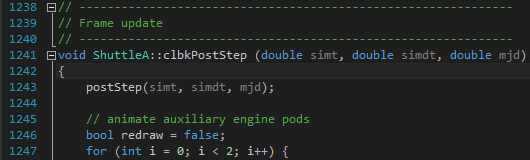
\includegraphics[width=1\textwidth]{img/post_step.png}
                \caption{Début de la fonction clbkPostStep, modifiée par nos soins.}
            \end{center}
        \end{figure}
        

    \subsubsection{Javacc}
        Ayant réalisé en parallèle de l'étude pratique un projet compilateur, il nous a semblé naturel de réutiliser les mêmes outils, à savoir Javacc. Ceci nous a permis de gagner un temps précieux sur la prise en main de l'outil principal de développement.

        Javacc est un compilateur de compilateur, permettant de facilement créer un analyseur syntaxique, et de construire à partir de lui un analyseur sémantique et bien entendu, notre compilateur.
        
        La grammaire est définie dans un fichier \verb|.jj|\footnote{On y met aussi les appels vers les fonctions appropriées du compilateur au fur et à mesure que l'analyse syntaxique avance.}, puis Javacc se charge de générer du Java à partir de celui ci.
        
        \begin{figure}[!h]
            \begin{center}
                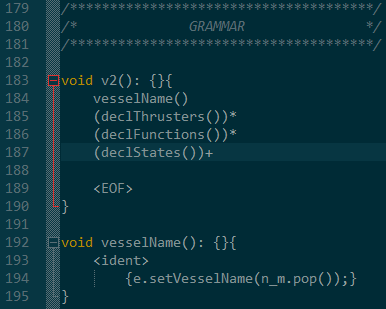
\includegraphics{img/grammar_jj.png}
                \caption{Début de notre grammaire du .jj.}
            \end{center}
        \end{figure}
        
        Il suffit ensuite de recompiler tout simplement le code généré avec le reste du compilateur, lui déjà écrit en Java.

    \subsubsection{Le langage}
        L'objectif était de garder un langage simple, avec des fonctionnalités limitées: pas de tableaux, pointeurs, et autres.

        Même si ce choix peut paraître étrange, on peut argumenter que complexifier le langage lui ferait perdre son intérêt\footnote{Rappelons qu'il s'agit d'un langage de démonstration, qui doit pouvoir être pris en main par des personnes n'ayant jamais programmé ou presque.}, puisqu'il suffirait d'apprendre directement le C++ et ne plus être limité par notre langage pour réaliser des controleurs plus complexes.
        
        Ci-dessous la grammaire presque complète (certaines parties étant suffisamment explicites, nous ne les détailleront pas).

        \begin{Verbatim}[frame=single]
Automata = VesselName()
           ThrusterDeclaration()*
           FunctionDeclaration()~
           StateDeclaration()~
           EOF
VesselName = <ident>
ThrusterDeclaration = <ident> ":" <ident>
FunctionDeclaration = Type() <ident> "(" Args() ")" "{"
                          Instruction()*  
                      "\}"  
StateDeclaration = <ident> "\{"
                       Instruction()* 
                   "\}" 
Instruction = DeclVar()
              | Affect()
              | FctCall()
              | If() 
              | While() 
              | Return()
              | Gotogoto() 
              | ApiGet() 
Gotogoto() = "GOTOGOTO" <ident>
ApiGet= "API\_GET" "{" 
            Getter()*
        "}"
Getter =  Dests() "=" <ident> "(" Args() ")" ";"
Dests =  <ident> (( "," <ident>)*)?
        \end{Verbatim}

        Cette grammaire a été réduite au maximum (on aurait pu par exemple interdire les return directement dans la grammaire), et ne suffit pas à interdire tout les abus de l'utilisateur. Ce travail est laissé à l'analyseur sémantique, qui s'assure de la cohérence et la validité des opérations demandées.
        
        On peut remarquer l'étrangeté d'ApiGet. Il s'agit d'une conséquence d'un choix technique, qui visait à rendre la récupération des informations sur le vaisseaux simple. 
        
        Par exemple, lorsque l'on récupère la vitesse du vaisseaux, on va récupérer au total 3 doubles: la vitesse en \verb|x|, \verb|y|, et \verb|z|. Nous avons donc voulu obtenir une syntaxe de la forme \verb| x,y,z = GET_SPEED(); |, ce qui entrait en conflit avec les affectations habituelles\footnote{Une amélioration possible (mais difficile techniquement à mettre en place) pourrait être la généralisation du renvois multiple, par exemple avec la création d'un type n-uplet.}.
        
        \subsubsection{Compilation de l'automate}
            Après avoir écrit l'automate dans un fichier \texttt{.mw}, nous pouvons donc le compiler.
            
            Notre compilateur prend trois arguments:
            \begin{itemize}
                \item le fichier source (obligatoire)
                \item le fichier \verb|.cpp| de sortie (optionnel, \texttt{Automata.cpp} par défaut)
                \item le fichier \verb|.h| de sortie (optionnel, \texttt{header.h} par defaut)
            \end{itemize}
            
            Alors que \texttt{Automata.cpp} sera à intégrer tel quel dans le projet, \texttt{header.h} contient le code qui doit être copié dans le \texttt{ShuttleA.h}, et ne doit pas (et ne peut pas) être utilisé en l'état.

        \subsubsection{Recompilation du vaisseau}
            Le code généré, nous pouvons maintenant recompiler le vaisseau, afin de tester l'efficacité de l'automate.
            
            Il faut donc rajouter au projet VisualStudio le fichier contenant le code (\texttt{Automata.cpp}), et coller les entêtes des fonctions dans son header.
            
            Pour cette deuxième partie, deux solutions:
            \begin{itemize}
                \item Le faire manuellement, à partir de \texttt{header.h};
                \item Ou bien laisser un outil les coller automatiquement, pour peu que l'on ai rajouté des "tags" dans le header à l'endroit voulu. 
            \end{itemize}
            
        \begin{figure}[!h]
            \begin{center}
                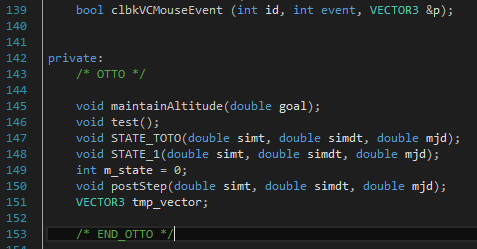
\includegraphics{img/code_header.png}
                \caption{Code de l'automate collé entre les tags.}
            \end{center}
        \end{figure}
        
            Le projet peut maintenant être recompilé par Visual Studio, et le lancement du vaisseau peut être regardé depuis son canapé, puisque qu'aucune entrée utilisateur est nécessaire.
            
    \subsection{Résumé de la procédure}
        \paragraph{Adapter le vaisseau}
            \'Etape à faire qu'une seule fois, il suffit de rajouter l'appel à la fonction mère de l'automate dans le corps de la fonction \verb|clbkPostStep| du vaisseau, ainsi que des tags dans le header pour pouvoir y coller automatiquement le code généré.
            
        \paragraph{(Ré)écrire l'automate} en utilisant la grammaire définie.
        
        \paragraph{Compiler cet automate} et coller le résultat dans le vaisseau adapté
        
        \paragraph{Recompiler le vaisseau}
            

    \subsection{Objectifs atteints}
        Le langage et sa grammaire ont été défini, et possèdent un compilateur qui produit du C++ valide et compatible avec l'API d'Orbiter.
        
        Cela nous a permis d'écrire plusieurs automates (ayant toutes des taches basiques) et de faire voler notre ShuttleA en auto-pilote.

    \subsection{Améliorations possibles}
        Plusieurs améliorations sont possibles à l'avenir, et peuvent constituer suffisamment de travail pour potentiellement en faire un nouveau sujet d'étude pratique dans les années futures.
        On peut lister par exemple:
        \begin{itemize}
            \item La suppression de la dépendance à Visual Studio, pour avoir une chaîne logicielle complète.
            \item Avoir un plus grand nombre de vérifications lors de la compilation de l'automate. Dans l'absolu, si le compilateur C++ produit une erreur (ou un warning), notre compilateur devra avoir affiché une erreur/warning en premier lieu.
            \item Généraliser l'utilisation des n-uplets\footnote{Qui pour l'instant sont une fonctionnalité plus exotique, réservée aux API\_GET}, ce qui permettrait par exemple d'avoir le retour de multiples valeurs pour une fonction.
            \item \og Couper \fg{} l'automate quand l'utilisateur reprend le contrôle manuel du vaisseau.
            \item Supporter un plus grand nombre de vaisseaux, en retravaillant un peu la grammaire et l'intégration du code.
            \item \'Ecrire de nouveaux automates pour les démonstrations lors d'expositions ou de conférences .
            \item Ajouter une GUI permettant de choisir son vaisseau et son automate.
        \end{itemize}

\section{Conclusion}
    Bien que les principaux objectifs aient été atteint, des finitions sont toujours possibles, et même souhaitable.
        
    Travailler sur ce simulateur nous a vraiment plus. Quelle fierté lorsque notre Shuttle A a fini par s'élever tout seul. 
    Ce projet permet de croiser un domaine très théorique (la théorie du contrôle) avec quelque chose de concret (une fusée qui décolle). C'est cela qui rend ce projet valorisant et passionnant.
    
    Le travail sur celui-ci mérite d'être continué, afin de produire à terme, une véritable vitrine de démonstration pour la théorie du contrôle.


\end{document}
